\subsection{Overview}
The TrackMe services are built on a client-server structure, this way the system is organized through abstraction levels.
We chose to adopt a 3-tier architecture:

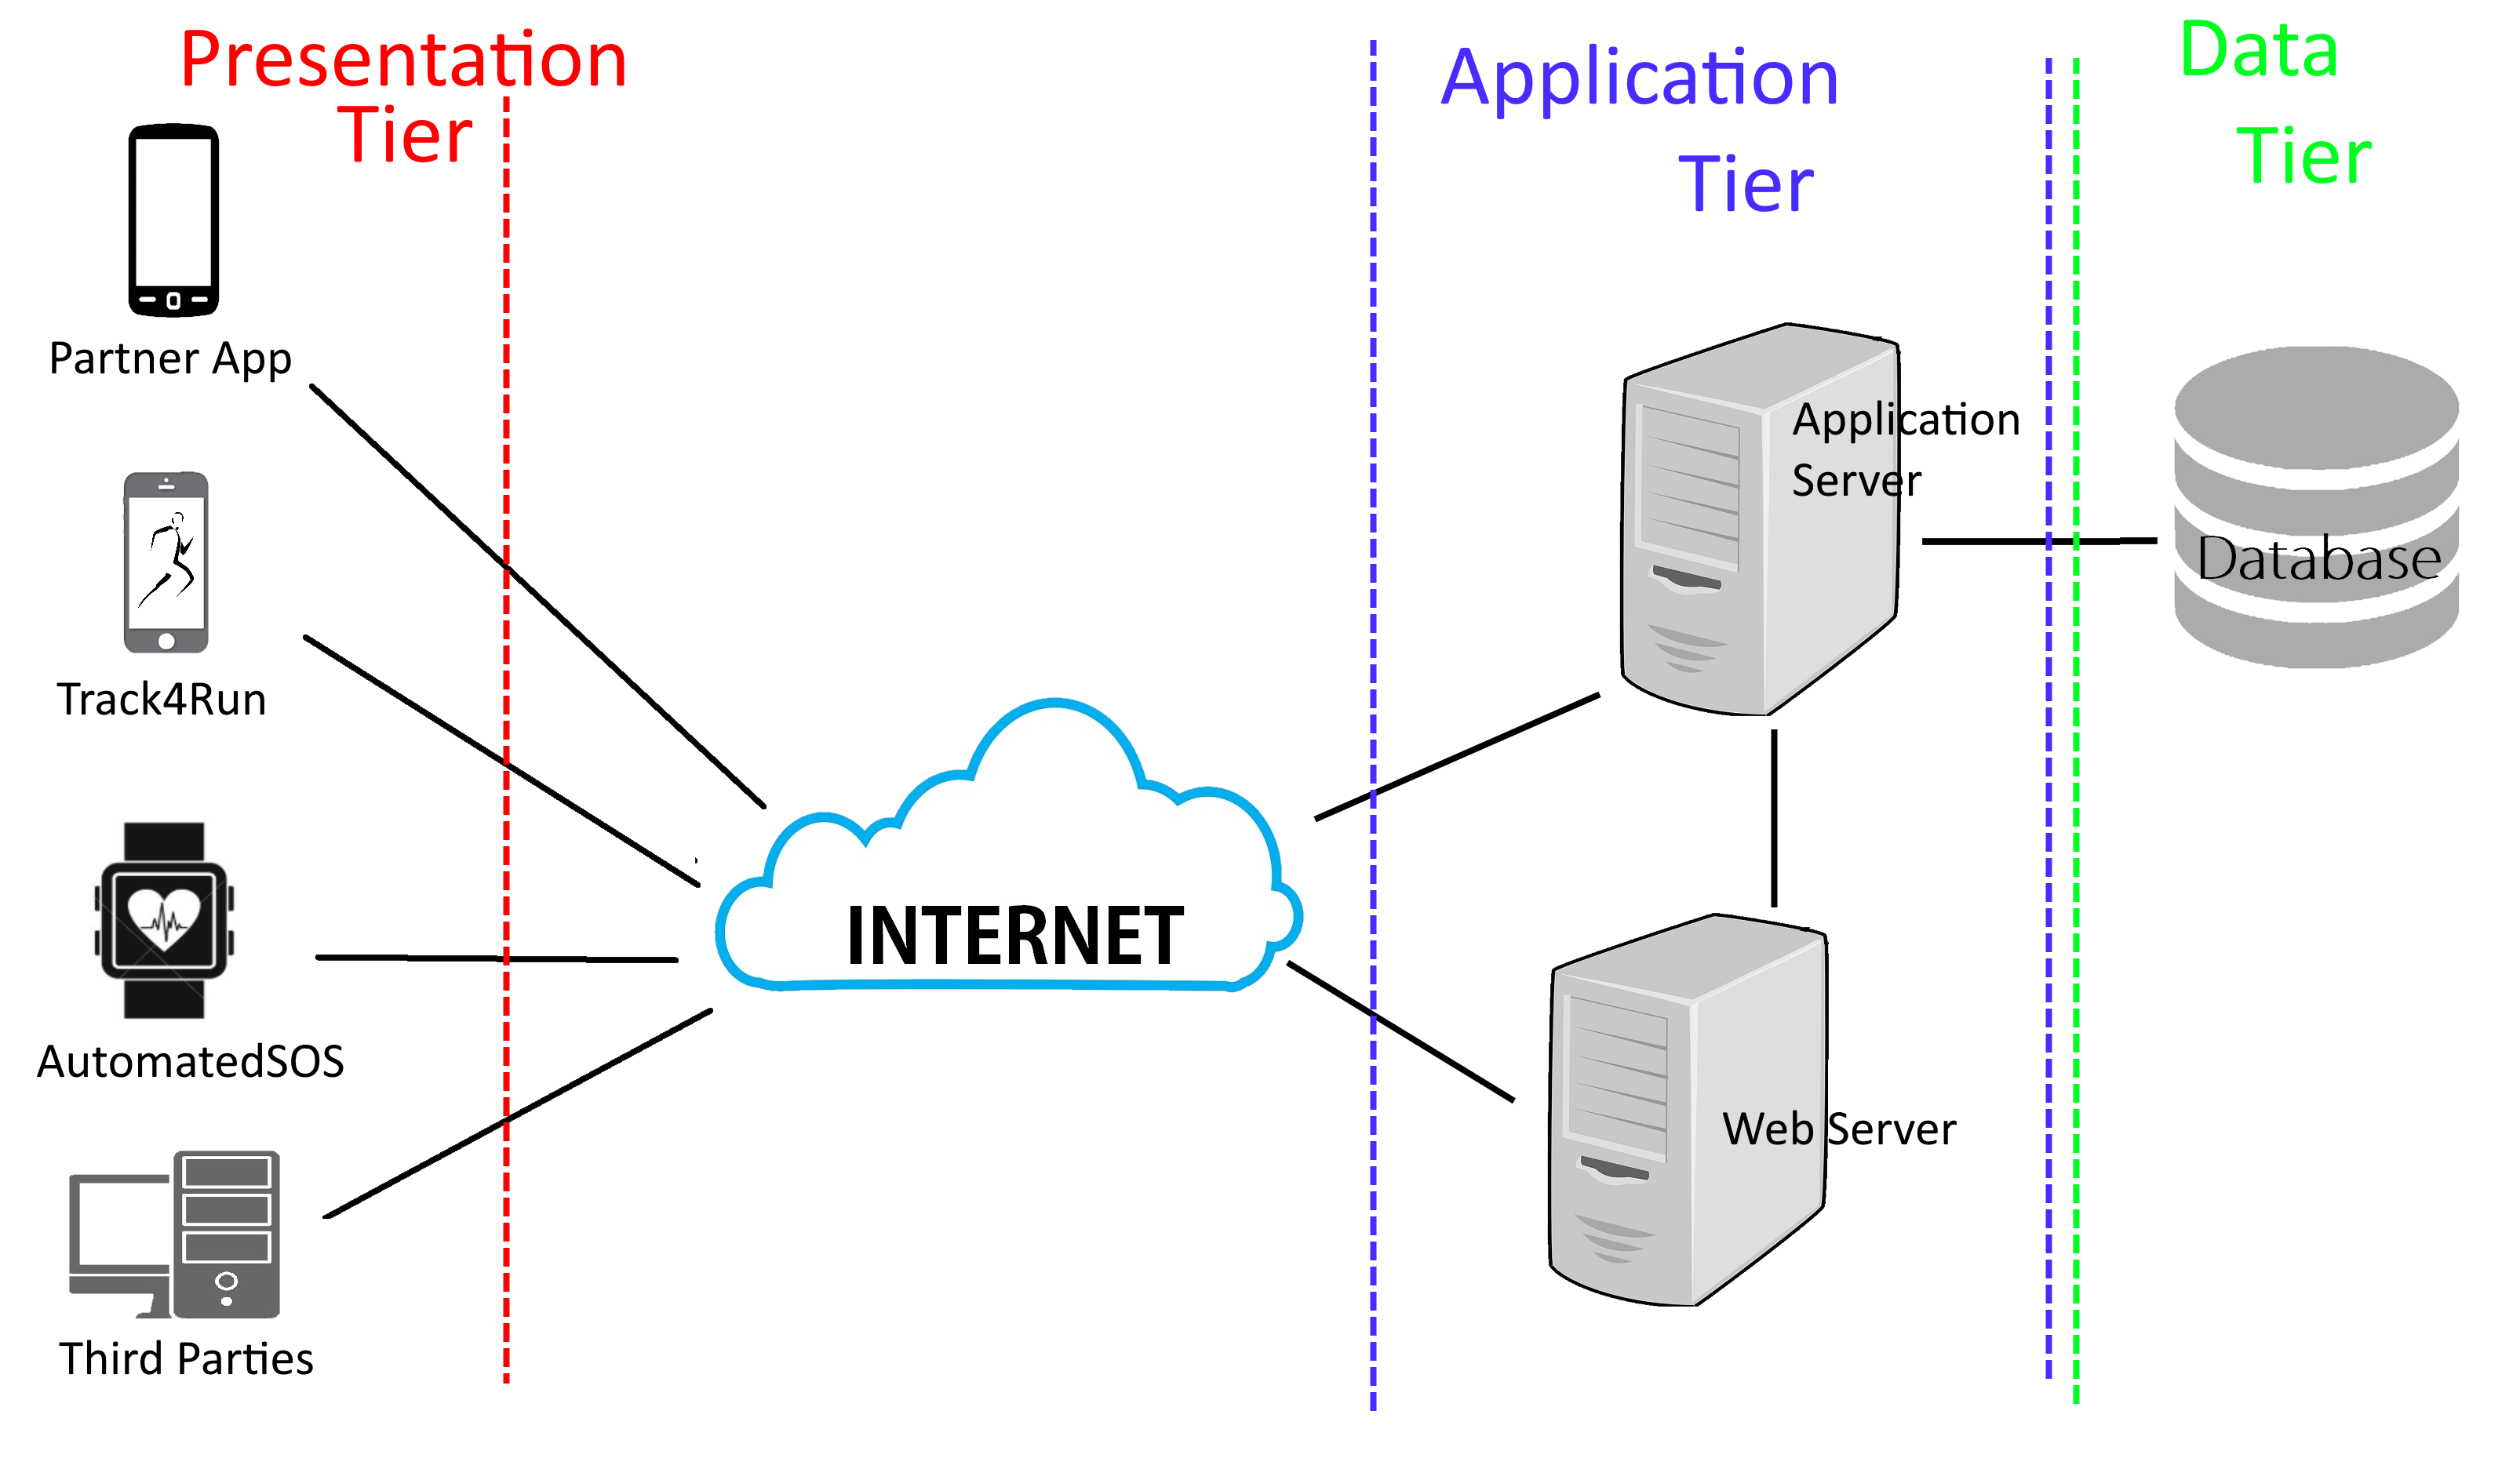
\includegraphics[scale=0.2]{Images/Overview.png}

\begin{itemize}
	\item \textbf{Presentation Tier} \\This layer makes the interaction possible between the user and the system. Here the user sees all the information provided by the system in a easily way to understand them.
	\item \textbf{Application Tier} \\This layer is managed almost totally by Data4Help service that is in charge of:
	\begin{itemize}
		\item store data incoming from the external;
		\item collect data information from database in order to execute Third parties’ requests;
		\item also generates data statistics on data collected;
		\item send to third parties requested data.
	\end{itemize}
	Moreover even AutomatedSOS has logic application in order to continuously monitor users’ health status.
	\item \textbf{Data Tier} \\In this layer all the sensible users’ data (location, health status) are stored into Databases and are retrieved by the application tier in order to do statistics and answer third parties’ requests.
\end{itemize}

More specifically Data4Help manage the data and core logic sections while AutomatedSOS and Track4Run manage the presentation section. Actually, a small part of application tier is also present in AutomatedSOS, this is due to the fact that the Health Monitoring process requires to be executed as fast as possible.

\clearpage
\subsection{Component View}

\subsubsection{Component Diagram}
\begin{figure}[H]
\centering
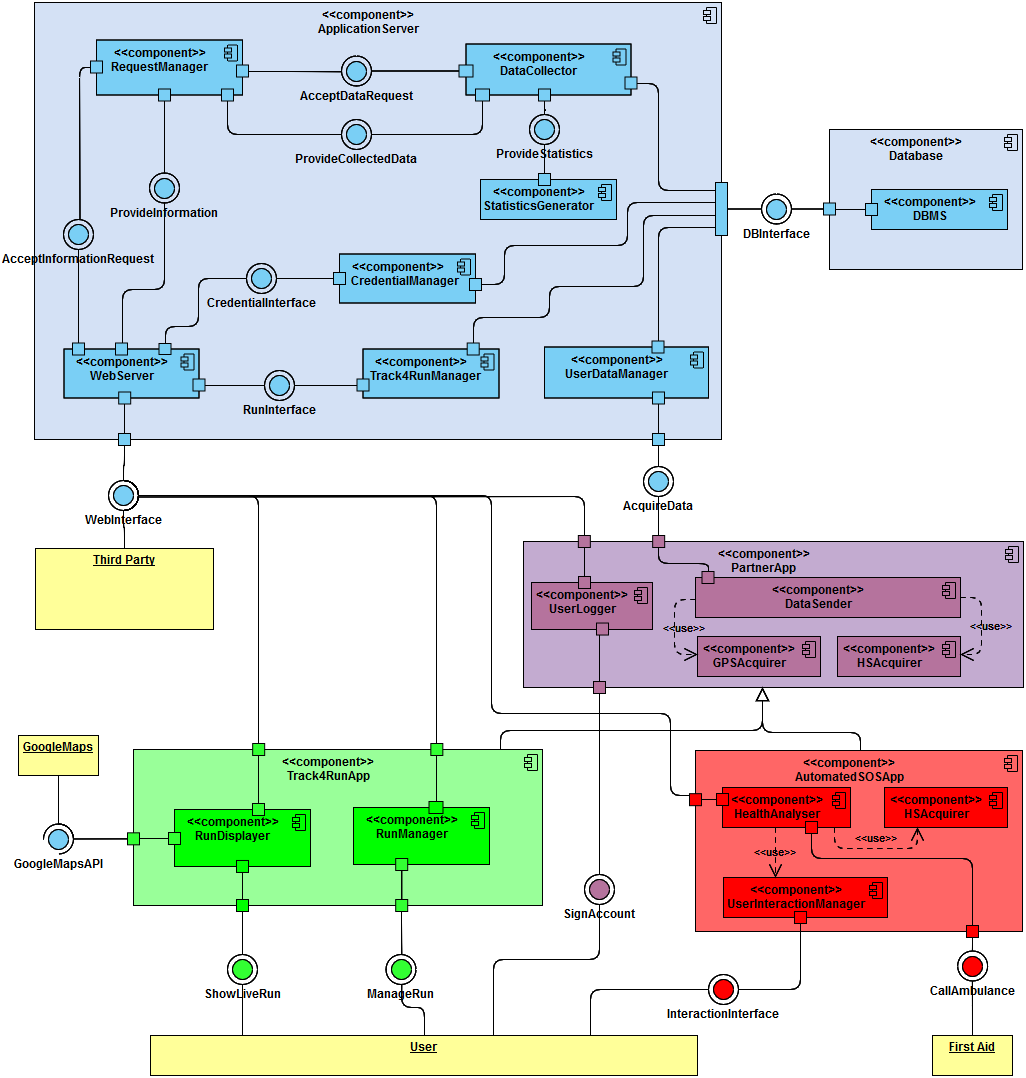
\includegraphics[scale=0.44]{Images/ComponentDiagram.png}
\caption{Component Diagram}
\end{figure}

{\large \textbf{Component diagram description}}
\begin{enumerate}
\item [1] \textbf{ApplicationServer} 
This huge component is in charge of manage Data4Help services so store and provide, for interested companies, users’ data (such as GPS location and daily Health Status). Moreover it manages race information of Track4Run application.

	\begin{enumerate}
	\item [1.1] \textbf{WebServer:} In order to accept and supply information to who need them, this component offer a friendly web interface to simplify these operations
		
	\item [1.2] \textbf{RequestManager:} In order to support web server in its job, this component manage all the incoming request: it sorts them per urgency, it wrap the request in a smart data structure and send it to Data Collector, it unwrap the answer from Data Collector and it continuously generates data exchange if a live acquisition is active
		
	\item [1.3] \textbf{DataCollector: } This component is in charge to communicate with Database in order to retrieve information and supply them to Request Manager. To perform these operations the component should receive request from Request Manger, unwrap it, creates a query to database that cover the question and send it to database; once the database has responded it should wrap the answer and provide it to Request Manager. Moreover if a statistic on data is required it requires it to Statistic Generator.
		
	\item [1.4] \textbf{StatisticGenerator: } This component is in charge of generates statistic on data provided by data collector such as arithmetic mean, variance from average, standard deviation and median.

	\item [1.5] \textbf{UserManager: } This component is in charge to communicate with users' device in order to log (or sign up) user and retrieve data collected.

	\item [1.6] \textbf{Track4RunManager: } This component is in charge to communicate with Track4Run applications in order to allow promoter to manage races.
	
	\item [1.7] \textbf{CredentialManager: } This component is in charge to communicate with the Web Server in order to enroll a user in the system and to check if the credentials inserted are corrected when a user wants to log in.
	
	\end{enumerate}
	
\item [2] \textbf{Database} 
This component is in charge of store physically data and organize them in a smart way according to DBMS rule, moreover it allows the access to those data.

	\begin{enumerate}
	\item [2.1]\textbf{DBMS: }
	This component is in charge of store all the data involving the system, from users' parameters, third parties' requests and races' information generated by Track4Run application
	\end{enumerate}
	
\item [3]\textbf{PartnerApp: }
This component implements how the application partner of TrackMe is basically structured, from the components in charge of retrieve raw data from device's API to who is in charge to communicate with the Main Server. This component is extended by all the partner applications that want to exploit Data4Halp service, so even by AutomatedSOS and Track4Run.

	\begin{enumerate}
	\item [3.1]\textbf{GPSAcquirer:}
	This component is developed in order to acquire GPS location from user's device at constant time period.
	
	\item [3.2]\textbf{HSAcquirer:}
	This component is developed in order to acquire Hearth rate, Blood pressure and Calories consumed from user's device at constant time period. (Obviously if device support it). 
	
	\item [3.3]\textbf{UserLogger:}
	 This component offers to client the possibility to become Data4Help user, so it is in charge to show to client the policy to accept and acquire all the credentials inserted during registration. Moreover has to communicate to Main Server the registration of a new user.
	 
	\item [3.3]\textbf{DataSender:}
	This component, exploiting GPSAcquirer and HSAcquirer features, is in charge to provide to UserManager component inside main server all the retrieved data whenever are ready to be sent.
	\end{enumerate}

\item [4]\textbf{AutomatedSOSApp: }
This component should extend all that is specified in partner application component to exploit all its features. AutomatedSOS component,also, has to use (as Data Sender) the HSAcquirer in order to check health status parameter and call the first aid whenever is required.

	\begin{enumerate}
	\item [4.1]\textbf{HealthAnalyser: }
	This component exploiting HSAcquirer features is in charge to analyse continuously health parameters, compare last acquired data with historical data in order to improve the reaction time, check data in order to prevent user's diseases and call an ambulance whenever such parameters are below a certain threshold, compiling and providing also a special report.
	
	\item [4.2]\textbf{HSAcquirer:}
	This component is developed in order to acquire Hearth rate, Blood pressure and Calories consumed from user's device at constant time period. (Obviously if device support it). 
	
	\item [4.3]\textbf{UserInteractionManager:}
	This component is created in order to give to users the possibilities to see his/her current or historical health status parameters and to set preferences.
	\end{enumerate}
	

\item [5]\textbf{Track4RunApp: }
This component should extend all that is specified in partner application component to exploit all its features. Track4Run component,also, should provide to spectator the possibilities to select and spectate to a run,also allows promoter to create and manage a race providing all the useful information.
	
		\begin{enumerate}
	\item [5.1]\textbf{RunDisplayer: }
	 This internal component is in charge to provide a human interface to the user that allows him to specify the race that he want to spectate and then show the position of all the athletes in the race, exploiting Google Maps API.
	
	\item [5.2]\textbf{RunManager: }
	This internal component is in charge to provide to user the possibility to promote a run inside the system, date,path,name,maximum number of partecipants and description. Moreover a promoter can invite specific users providing their fiscal code. 
	\end{enumerate}
\end{enumerate}
\clearpage

\subsubsection{Entity Relationship Diagram}
\begin{figure}[H]
\centering
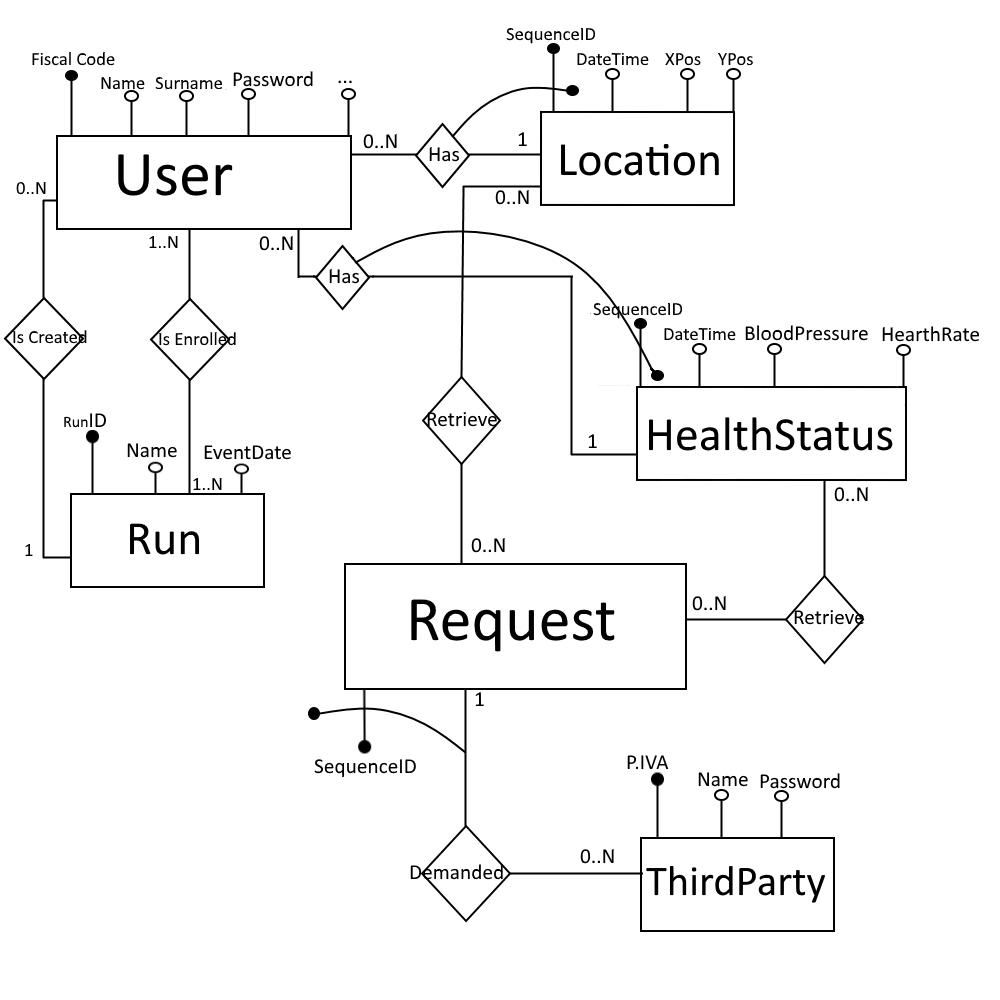
\includegraphics[scale=0.65]{Images/ERDiagram.png}
\caption{Entity Relationship Diagram Diagram.}
\end{figure}

\newpage
\subsection{Deployment View}
The following Deployment Diagram captures the topology of the system's hardware.
The SmartphoneApp and SmartWatchApp (Presentation Tier) communicate to the Application Server through RMI, while the WebBrowser communicates to the WebServer through HTTP protocol. The Application Server (Application Tier) communicates to the Database Server (Data Tier) through JDBC.

\begin{figure}[H]
\centering
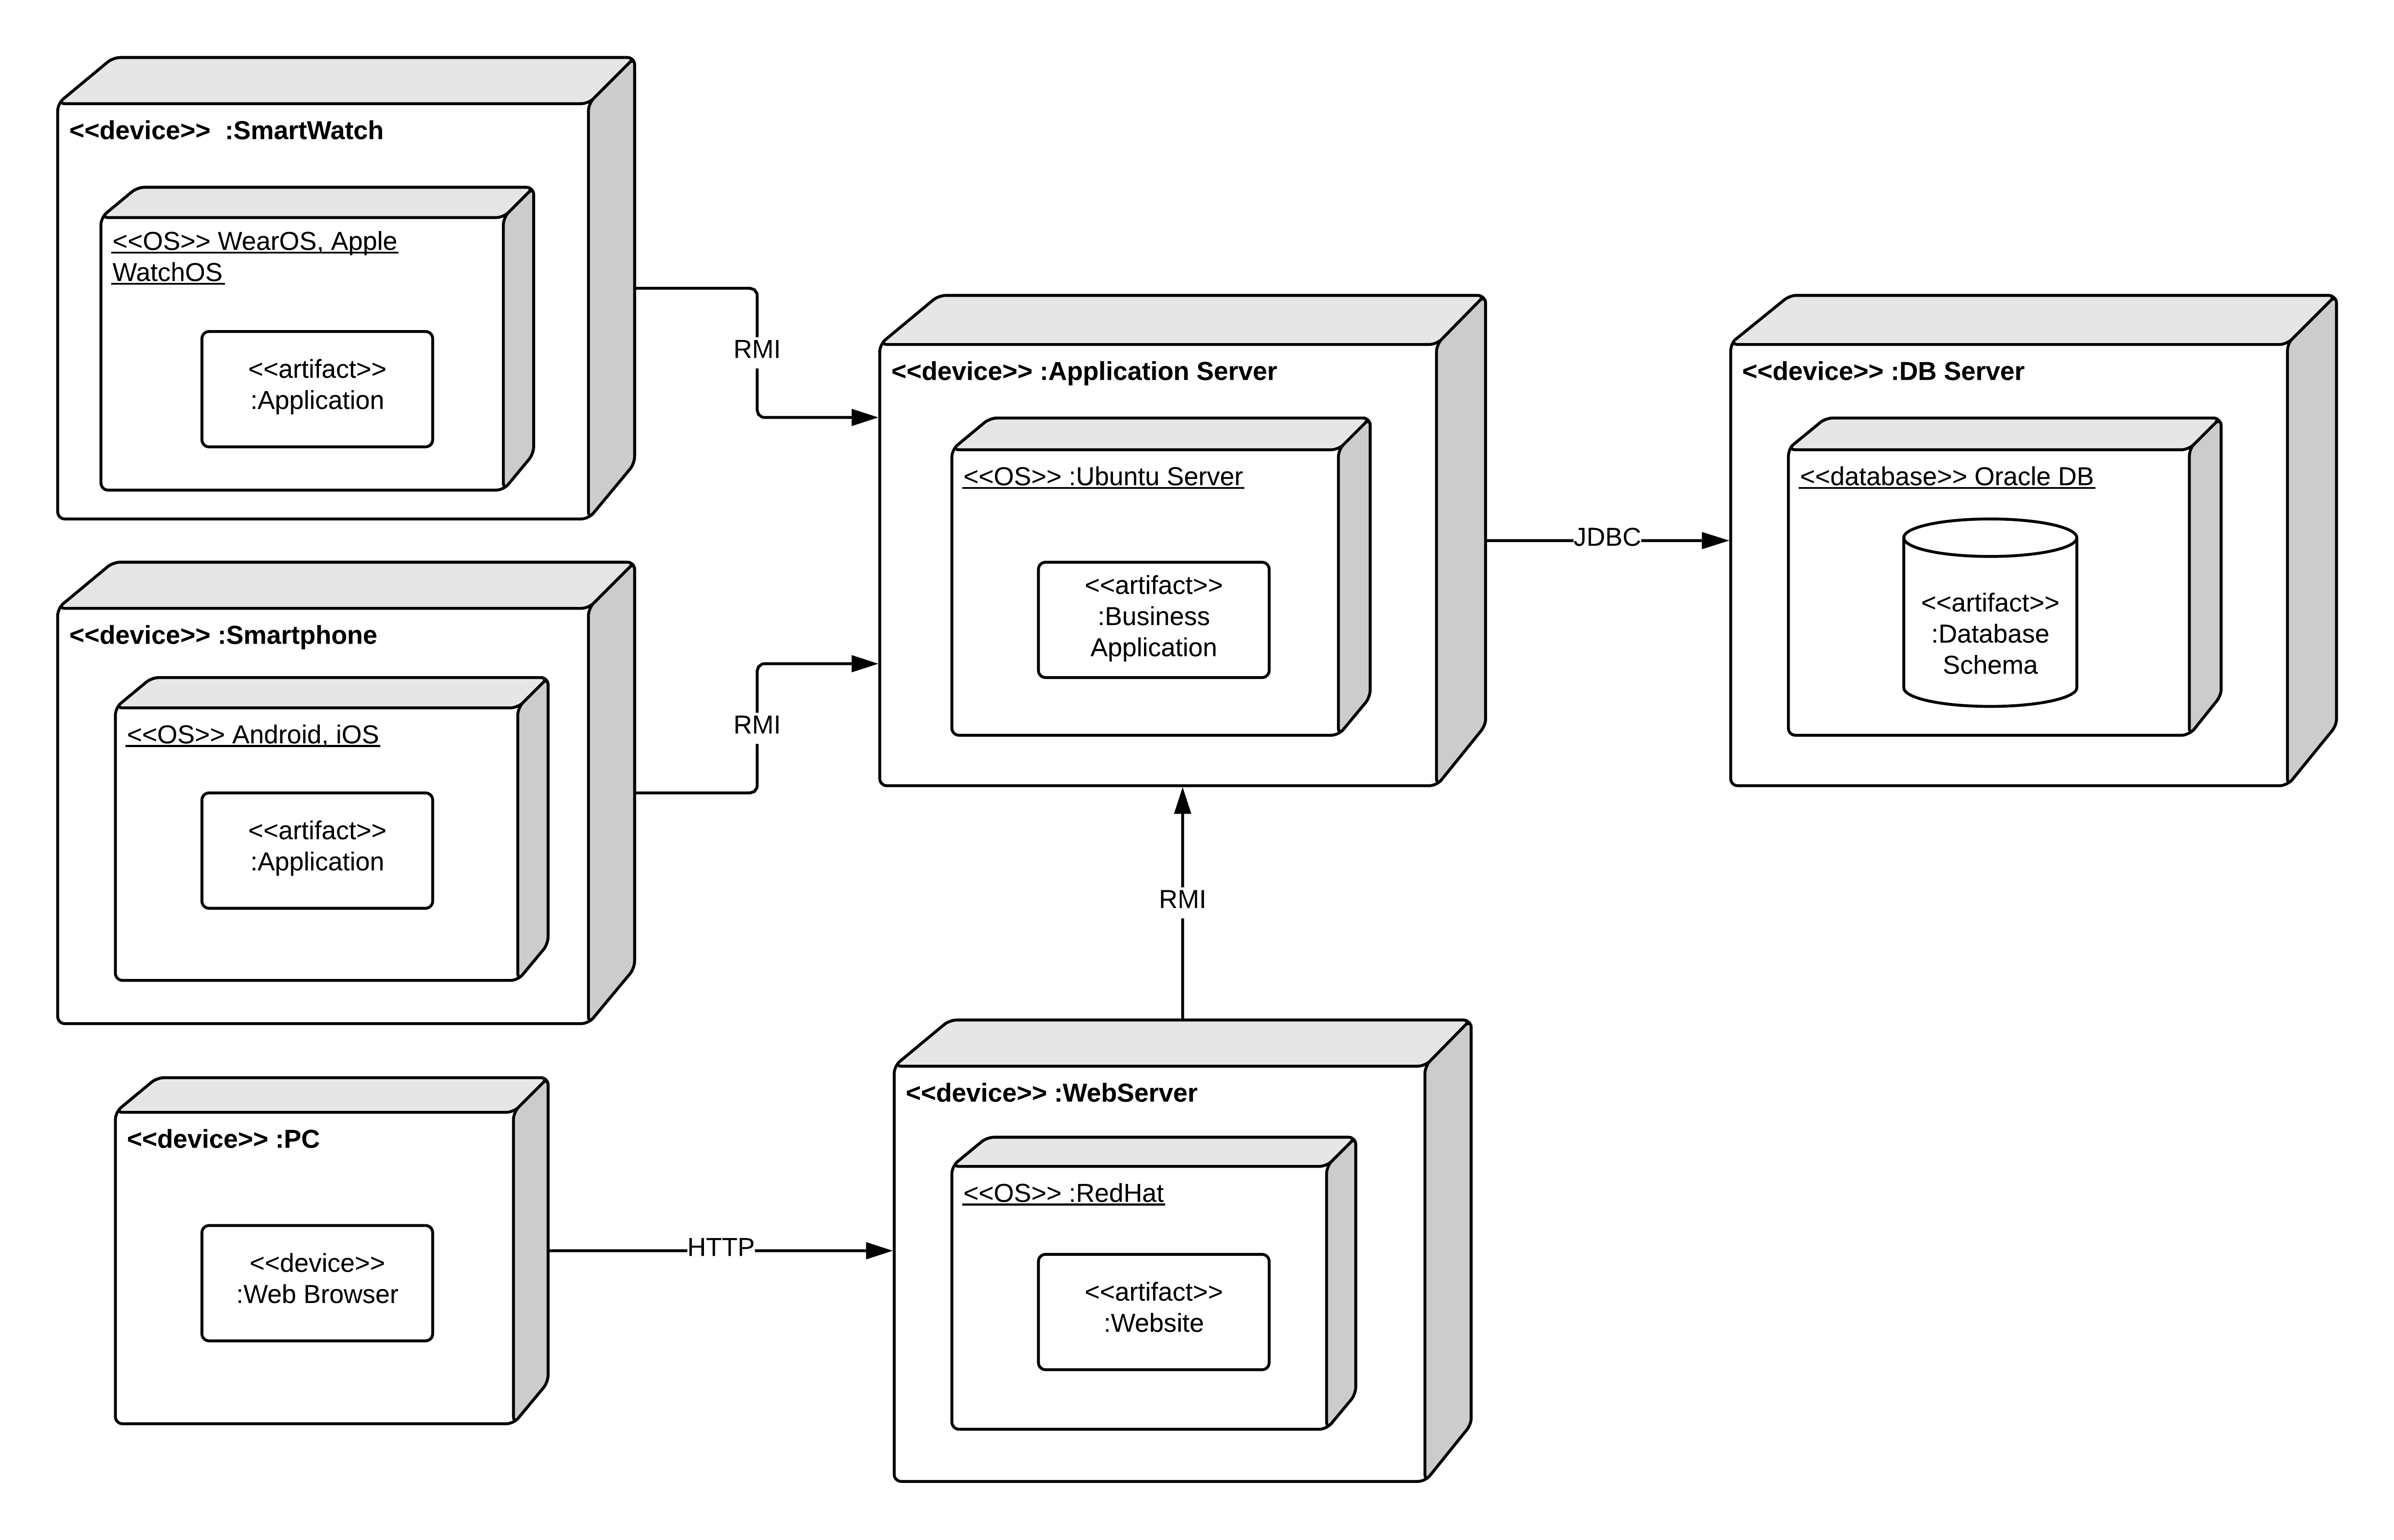
\includegraphics[scale=0.12]{Images/DeploymentDiagram.png}
\caption{Deployment Diagram.}
\end{figure}

\subsection{Runtime View}
In this section several Sequence Diagrams are shown in order to point up the interaction among components and their behavior in particular scenarios.
\newpage
\subsubsection{Individual Information Request}
The following Sequence Diagram shows the interaction between the components when a third party made a request to obtain individual information. Since the individual's security number provided by the third party in the request form cannot be associate to any real user (incorrect security number) or can be associate to a user that has not accept individual request privacy policy, the third party could get three different answers from the system.
\\[1.0cm]
\begin{figure}[H]
\centering
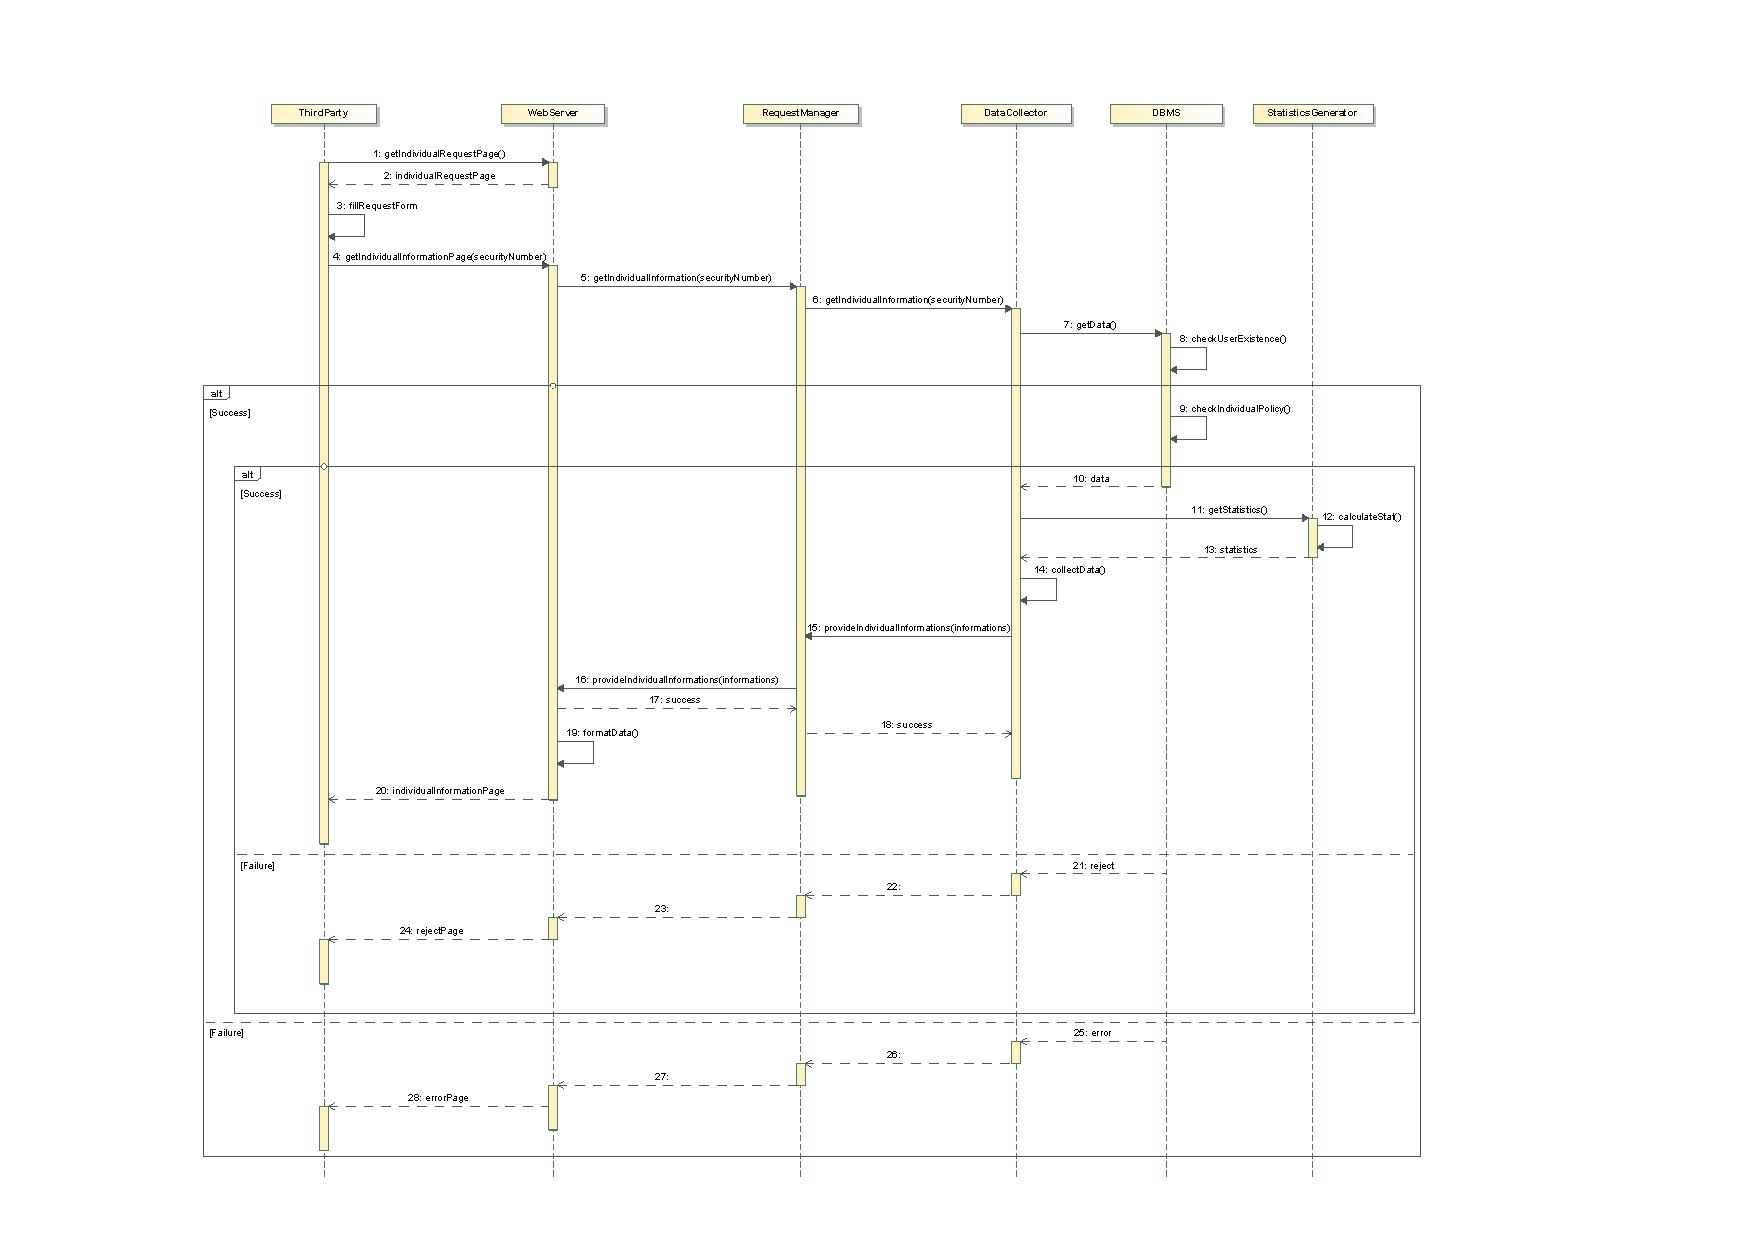
\includegraphics[scale=0.8, angle=0,origin=c]{Images/SequenceDiagrams/IndividualRequest.pdf}
\caption{Sequence Diagram n.1.}
\clearpage
\end{figure}
\newpage
\subsubsection{Send Ambulance Request}
In the below diagram is shown the interaction that the components have between each other to send an ambulance request to the first aid. The data retrieved by the GPS Acquirer and HealthStatus Acquirer both sent to Data4Help and sent to the HealthAnalyzer.
\\[0.5cm]
\begin{figure}[H]
\centering
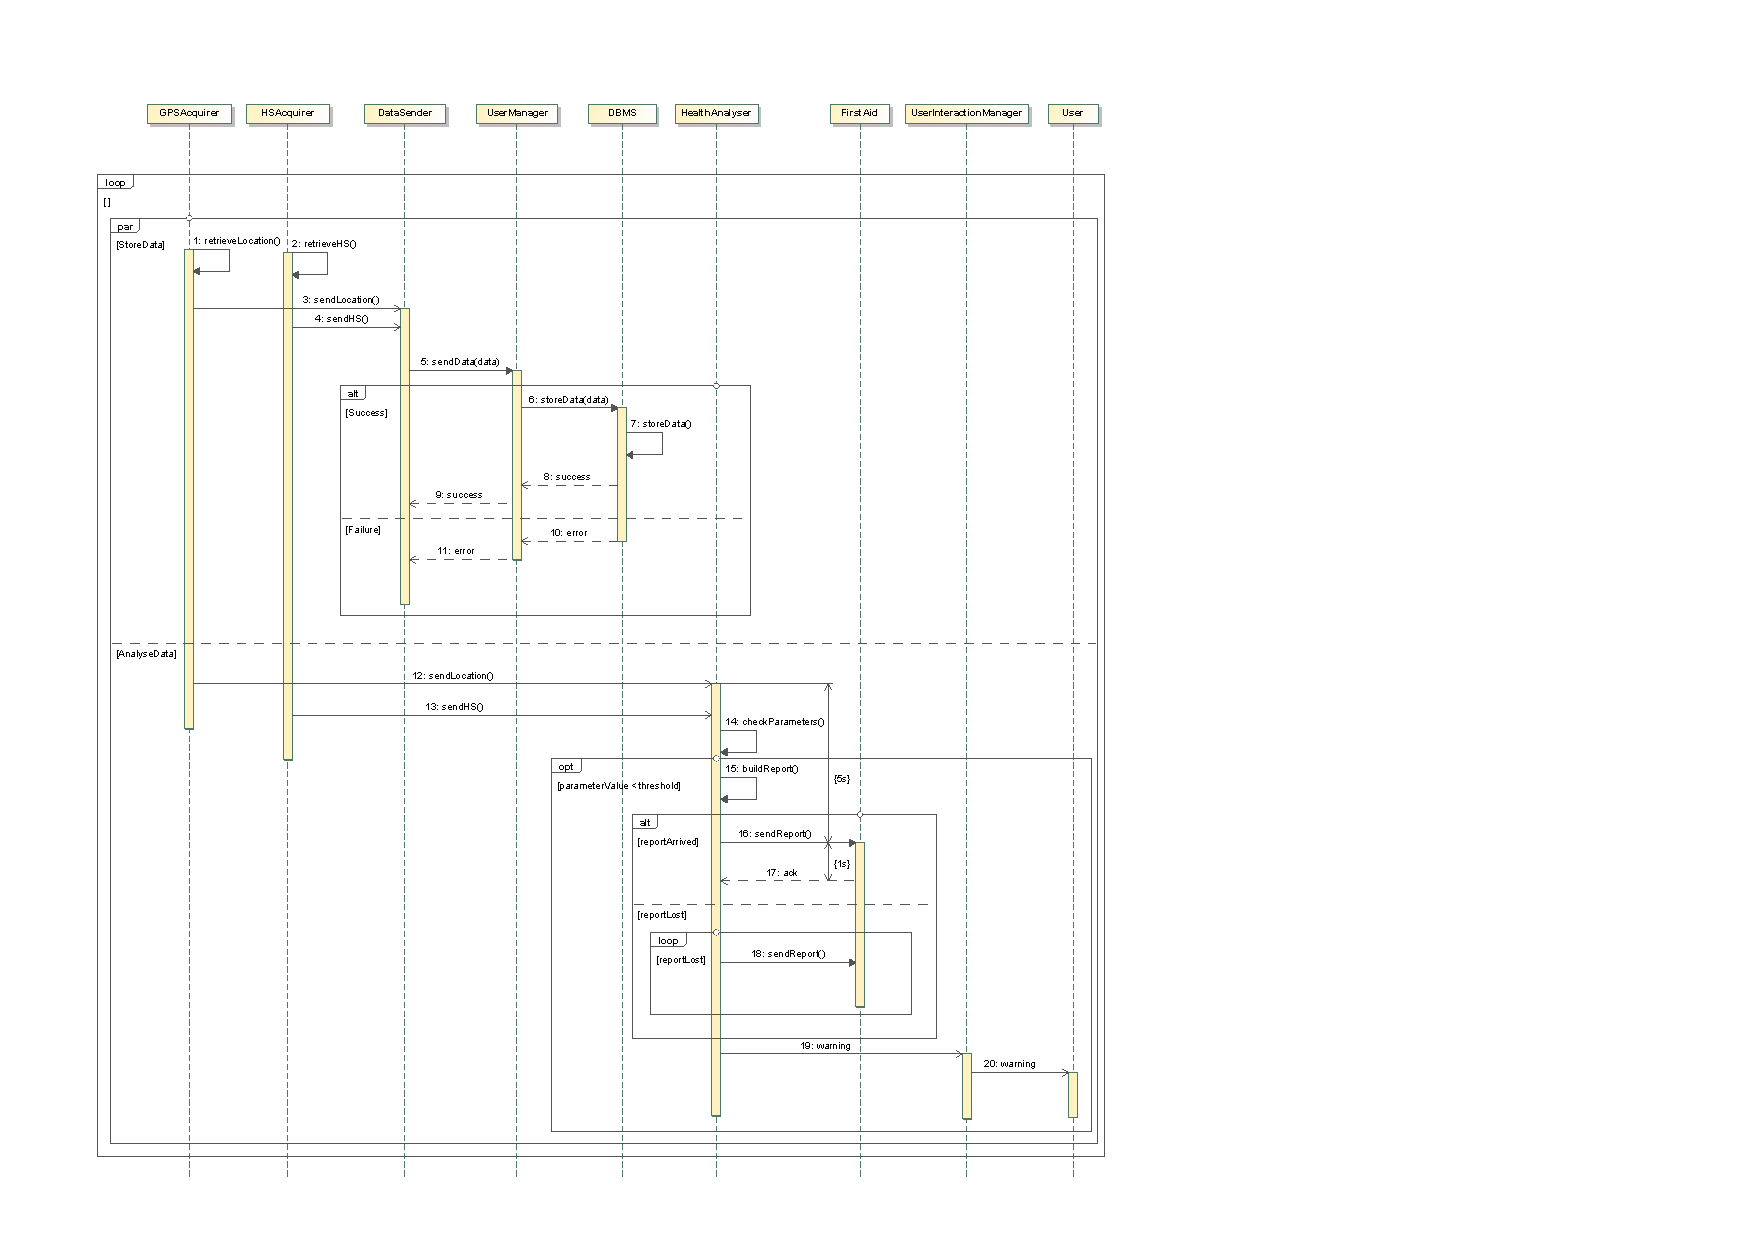
\includegraphics[scale=0.9, angle=90,origin=c]{Images/SequenceDiagrams/SendAmbulance.pdf}
\caption{Sequence Diagram n.2.}
\end{figure}
\newpage
\subsubsection{Spectate to a Run}
The next Sequence Diagram represents the interaction that the components have between each other to show the live positions during a run event, the chart starts at the moment when the user, already logged in, select a specific run to spectate.
\begin{figure}[H]
\centering
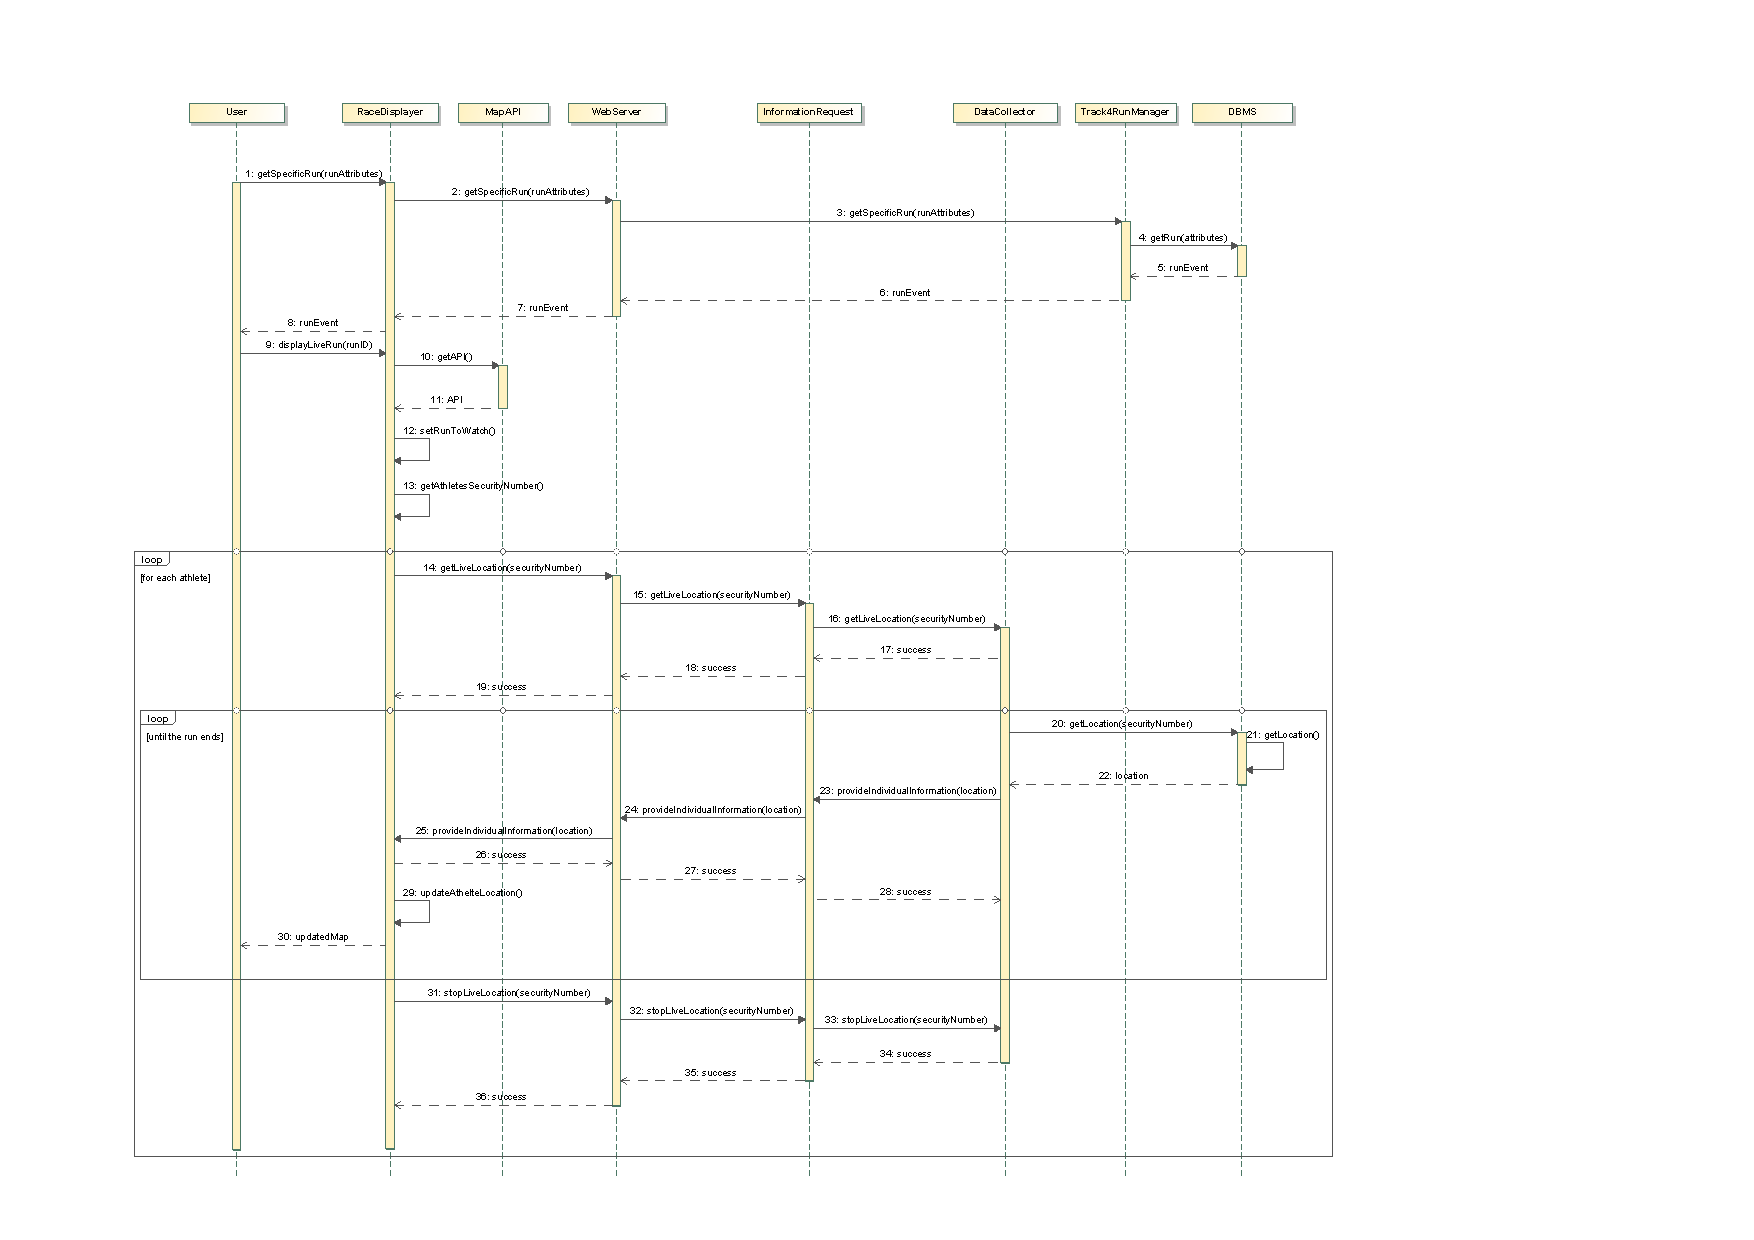
\includegraphics[scale=1, angle=90,origin=c]{Images/SequenceDiagrams/SpectateRun.pdf}
\caption{Sequence Diagram n.3.}
\end{figure}
\clearpage


\subsection{Component Interfaces}
\begin{figure}[H]
\centering
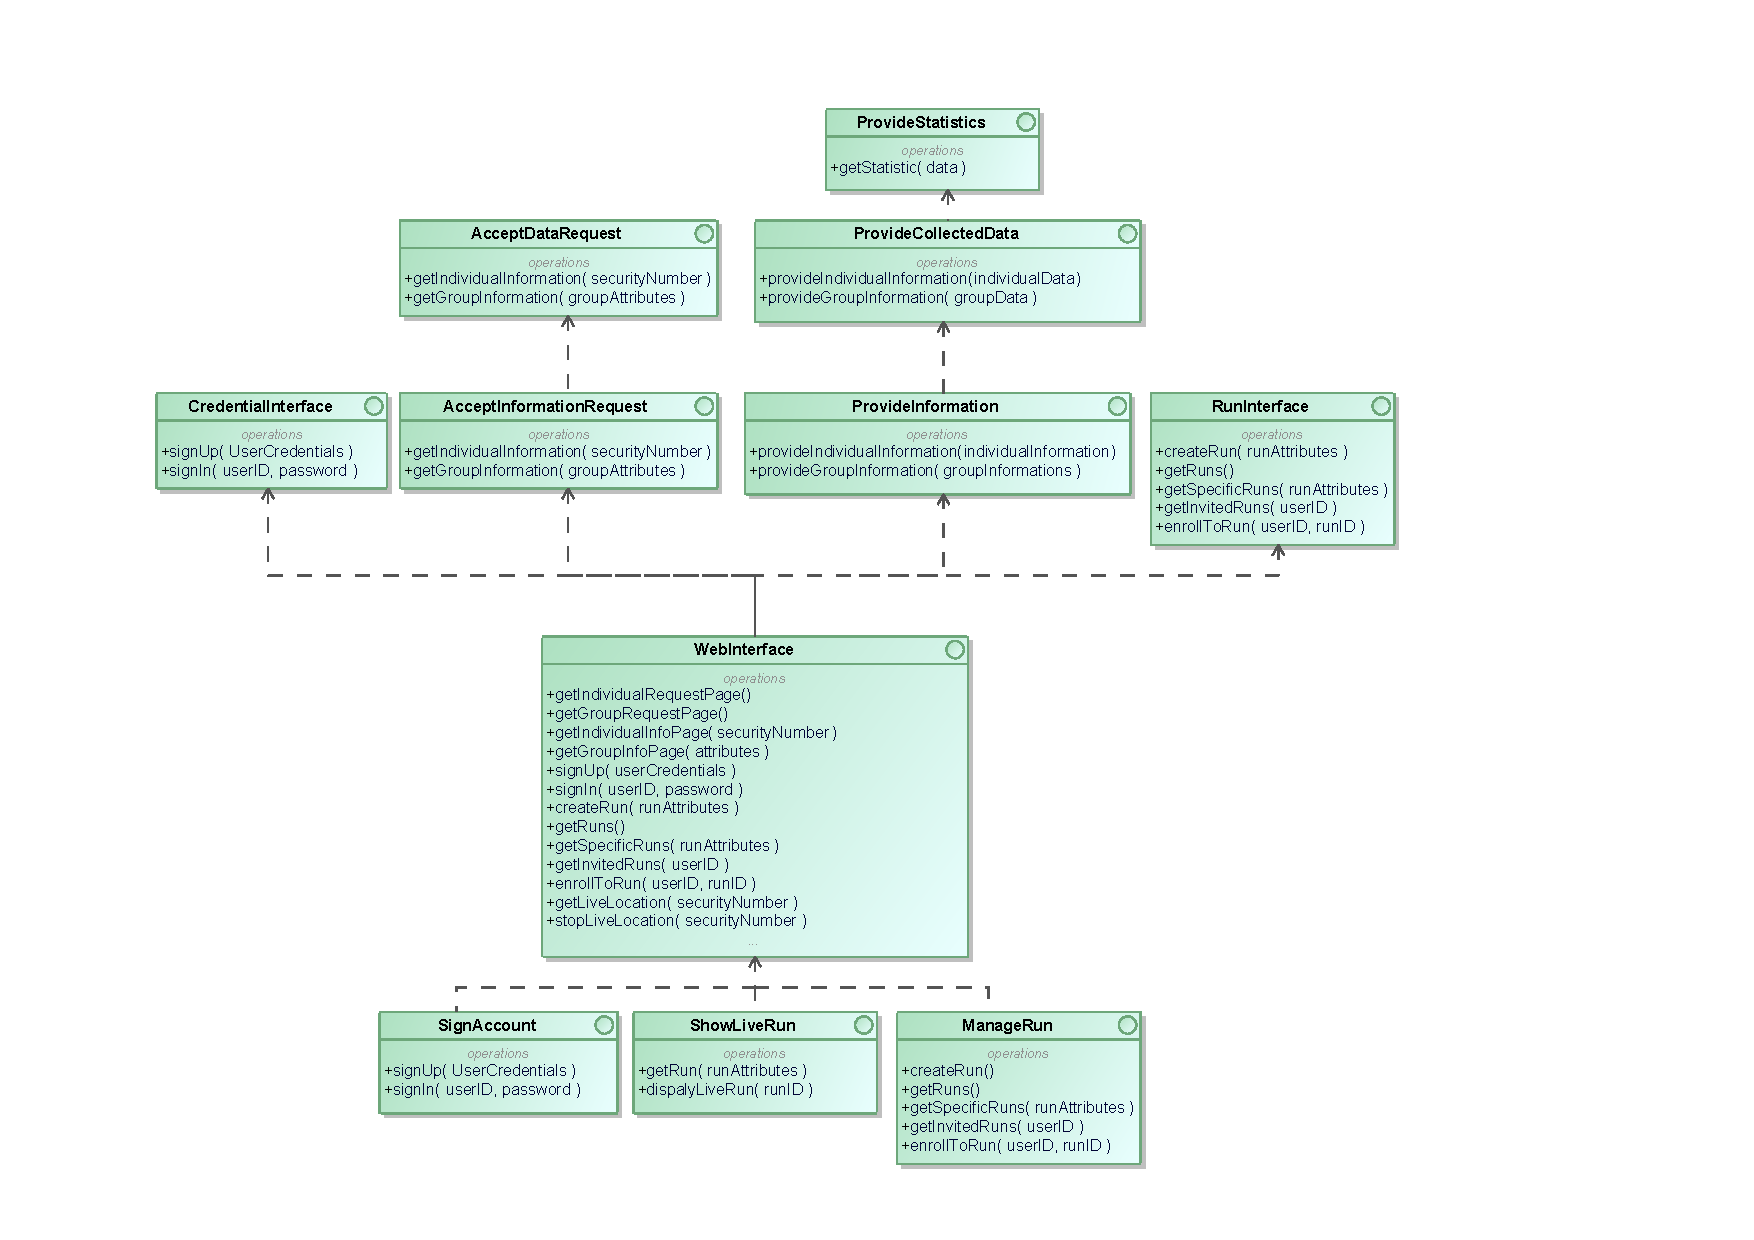
\includegraphics[scale=0.8, angle=0,origin=c]{Images/ComponentInterface.pdf}
\caption{Component Interfaces Diagram}
\end{figure}
\begin{enumerate}

\item[1.1] \textbf{WebServer: }
	\begin{enumerate}
		\item[1.1.1] \textbf{WebInterface:} Human interface for third parties that want to log in or retrieve information from Data4Help service. Software interface for Track4Run and for AutomatedSOS in order to provide requested information.
	\end{enumerate}
	
\item[1.2] \textbf{RequestManager: }
	\begin{enumerate}
		\item[1.2.1] \textbf{AcceptInformationRequest:} Software interface that allows WebServer to submit requests to be evaluated.
		\item[1.2.1] \textbf{ProvideInformation:} Software interface that provides to web server information answers that match previous requests.
	\end{enumerate}

\item[1.3] \textbf{DataCollector: }
	\begin{enumerate}
		\item[1.3.1] \textbf{AcceptdataRequest:} Software interface offered by DataCollector that accept requests from RequestManager formatted in the proper way.
		\item[1.3.1] \textbf{ProvideInformation:} Software interface offered by DataCollector that provide to Request Manager information answer formatted in the proper way.
	\end{enumerate}
	
\item[1.4] \textbf{StatisticGenerator: }
	\begin{enumerate}
		\item[1.4.1] \textbf{ProvideStatistics:} Software interface that provides statistic values to data collector. (The Software interface to receive data from Data collector to be managed is trivial and not explicitly specified).
	\end{enumerate}
	
\item[1.5] \textbf{UserManager: }
	\begin{enumerate}
		\item[1.5.1] \textbf{AcquireData:} Software interface that allows partner application to send data acquired to Data4Help.
		\item[1.5.1] \textbf{Enroll user:} Software interface that allows partner application's users to become registered users into TrackMe's system.
	\end{enumerate}

\item[1.6] \textbf{Track4RunManager: }
	\begin{enumerate}
		\item[1.6.1] \textbf{EditRaceSettings:} Software interface that allows Track4Run application to create or modify races information.
	\end{enumerate}

\item[2.1] \textbf{UserDBMS: }
	\begin{enumerate}
		\item[2.1.1] \textbf{StoreUserData:} Software interface that allows to store users' data into the database.
		\item[2.1.2] \textbf{ProvideStoredData:} Software interface that allows to retrieve users' data already collected in the database.
	\end{enumerate}
	
\item[2.2] \textbf{Track4RunDBMS: }
	\begin{enumerate}
		\item[2.2.1] \textbf{StoreRaceData:} Software interface that allows to to store races' data with queries.
		\item[2.2.2] \textbf{ProvideStoredData:} Software interface that allows to retrieve users' data already collected in the database.
	\end{enumerate}
	
\item[3.3] \textbf{UserLogger: }
	\begin{enumerate}
		\item[3.3.1] \textbf{Enrollment:} Software interface that permits to inform Users' Manager that a new user is successfully enrolled and with which credentials.
	\end{enumerate}
	
\item[4.1] \textbf{HealthAnalyser: }
	\begin{enumerate}
		\item[4.1.1] \textbf{CallAmbulance:} Software interface that allows AutomatedSOS to call, through the internet or in the worst case through telephone call, First Aid whenever is necessary in order to provide help to user. Moreover it provides to FirstAid a special report on which parameters are critical.
	\end{enumerate}
	
\item[5.1] \textbf{RaceDisplayer: }
	\begin{enumerate}
		\item[5.1.1] \textbf{SelectRace:} Human interface that allows user to specify the race to be displayed.
		\item[5.1.1] \textbf{ShowLiveRace:}  Human interface that allows to provide to the end user a map in which all the athletes involved in the selected race are displayed.
	\end{enumerate}	

\item[5.2] \textbf{RaceDisplayer: }
	\begin{enumerate}
		\item[5.2.1] \textbf{ManageRace: } Human interface that allows user to create and manage a run providing all the useful information.
	\end{enumerate}		

\end{enumerate}
\clearpage



\subsection{Selected Architectural Styles and Patterns}

This system is designed to be a Client-Server application with three tier that well separate the different components as shown in Overview description in order to implement MVC software design pattern.

\begin{enumerate}
\item[•] \textbf{Architectural Design: }\\

	\begin{enumerate}
	\item[-] Client-Server architectural pattern is chosen because it is the most used and easily implemented communication pattern in fact, in our application, is the best one to supply on third parties information requests and to acquire data from users via internet. 
Regarding the acquisition of users’ data, is the smartphone that decides, when data are successfully collected from the device, to call Data4Help server in order to provide and store data, furthermore even third parties call Data4Help server first and then the exchange of the information can be proceed; these two operations are the main core of the service then is logic that client-server architecture will be the right choice. 

	\item[-]Three tier architecture should be implement to assure reuse and maintainability of the system, in fact this division can permit to change some parts of the system without reconfigure the entire solution.
	
		\begin{enumerate}
		\item[*] Presentation Tier, as described above, is in charge of display on final users screen a human interface that allows the interaction with our system. This tier is present only on users' device: regarding third parties the software that is in charge to display human interface will be his own browser so the exchanged information will be an HTML page on Http connection; instead, regarding users, the software will be the application that runs on the device that works on HTML pages as well; so for both the type of users the interface to the Application Tier is the WebServer that allocate the right page to the right target. In order to supply on this aspect the partner application (AutomatedSOS and Track4Run as well) will be developed in HTML (with the support of JS and CSS) that are web languages, this aspect make also the application multi platform so they can be launched on either iOS or Android devices. Http communication protocol will be used for both connection.
		\item[*] Application Tier, as described above, is in charge to acquire all the data incoming from users, to store them on Data Tier and to handle the request on viewing data. This Tier is present on the largest part on Application server but even AutomatedSOS has inside his software an application service. All the component inside this tier will be developed in Java, in particular the Web Server runs tomcat Java servlet that generates the html pages for Presentation Tier, acquire data that users submit and communicate through RMI with the business application that runs on the Application Server. The business application is the main core of Data4Help service, and is composed by all the other components inside ApplicationServer (as Request Manager,Data Collector,Statistic Generator..); is required that it can interface with Web server, in order to acquire the external requests, and then using the components described above supply the information required; furthermore is in charge to manage all the information of users, as login or registration,or manages Track4Run races. Another very important aspect is that this application has to  retrieve data from users implementing a daemon on a specific port and listening for a TCP/IP connection incoming from partner application in order to acquire users' data. As mentioned before even AutomatedSOS implements a small part of application tier inside his software that is in charge to continuously monitor health status acquired, compare it with old data and call an ambulance via web if there is a necessity filling out a form which are indicated all the critical parameters detected.
		
	\item[*] Data Tier, as described above, is in charge to store and provide informations. This tier is present only on Database Server that is an Oracle machine using SQL schemas. The database is divided in two parts, one regarding Data4Help service that stores and manages users' data: historical users' location and health parameters; the other one regarding Track4Run that stores races' information. This Tier offers an SQL interface that can be exploit by Business application using JDBC libraries that supports SQL functions. 
		\end{enumerate}
	
	\end{enumerate}

\item[•] \textbf{Software Pattern: }

	\begin{enumerate}
	\item[-] The MVC (Model-View-Controller) is the obvious software pattern that can be applied on three tier architecture because can split the entire software solution in the three main region: the Model implements all that is described in data tier, the controller all that is described on Presentation tier and View all that is described in Presentation tier. All these 3 groups communicates each others through the so called Adapter Pattern.
	\item[-] The Adapter design pattern is developed to create an interface that permits to the MVC groups to easily communicate each others using different languages or different operating system that is mandatory in our system. This pattern is the representation of what is described on Component Interface section.
	\item[-] Strategy design pattern can be so much useful in the implementation of RequestManager component because it can dynamically change how to handle request queue in order to supply efficiently on heavy request load.
	\item[-] Proxy design pattern is an obvious consequence of Web Server, because this component stay in the middle between the two tier and creates a sort mask  that obscure what is behind it and simplify a lot the Presentation Tier software that has only to display what Web server indicates	
	\end{enumerate}

\end{enumerate}


\subsection{Other Design Decisions}